\documentclass[tikz]{standalone} 
%\usepackage{adjustbox}% <--- not needed
\usetikzlibrary{arrows,
                chains,% <--- new
                decorations.markings,
                shadows, shapes.arrows,
                positioning,
                fit}

\tikzset{% <--- modified
    decision/.style = {diamond,draw, fill=mblue!50},
        line/.style = {draw, -stealth, thick},
        block/.style = {rectangle, draw,  text width=4 em, minimum height=10 mm,
                       align=center},
        block2/.style = {rectangle, draw,  text width=1.32 em, minimum height=10 mm,
                       align=center},
        bigarrow/.style = {single arrow, draw=mred, minimum height=3em, outer sep=0pt}
        }
\makeatletter
\tikzset{suspend join/.code={\def\tikz@after@path{}}}
\makeatother

\definecolor{morange}{RGB}{255,127,14}
\definecolor{mblue}{RGB}{31,119,180}
\definecolor{mred}{RGB}{214,39,40}
\definecolor{mpurple}{RGB}{148,103,189}
\definecolor{mgreen}{RGB}{44,160,44}

\begin{document}              
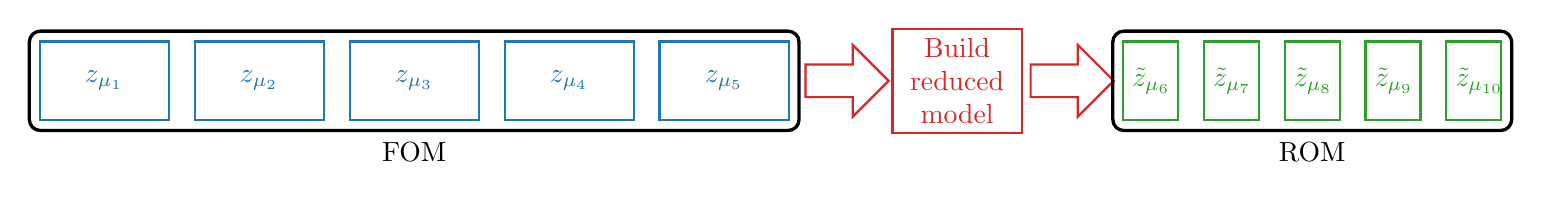
\begin{tikzpicture}[thick,
                        ]
\node [block, color=mblue] (A)  {$z_{\mu_1}$};% <-- A-1
\node [block, right=.3cm of A, color=mblue]  (B)  {$z_{\mu_2}$};
\node [block, right=.3cm of B, color=mblue]  (C) {$z_{\mu_3}$};
\node [block, right=.3cm of C, color=mblue]  (D) {$z_{\mu_4}$};
\node [block, right=.3cm of D, color=mblue] (E)  {$z_{\mu_5}$};% <-- A-5
\node [fit=(A)(E), label = below:FOM, draw, very thick, rounded corners] (expensive) {};
\node [bigarrow,
       right=0pt of E.east, xshift=.2cm] (arrow) {\vphantom{x}};
\node [block,suspend join, xshift=.5cm, right of=arrow, color=mred] (brm) {Build reduced model};
\node [bigarrow, right=0pt of brm.east, xshift=.1cm] (arrow2) {\vphantom{x}};
\node [block2, right of=arrow2, color=mgreen, xshift=.1cm] (A2)  {$\tilde{z}_{\mu_6}$};% <-- A-1
\node [block2, right=.3cm of A2, color=mgreen]  (B2)  {$\tilde{z}_{\mu_7}$};
\node [block2, right=.3cm of B2, color=mgreen]  (C2) {$\tilde{z}_{\mu_8}$};
\node [block2, right=.3cm of C2, color=mgreen]  (D2) {$\tilde{z}_{\mu_9}$};
\node [block2, right=.3cm of D2, color=mgreen] (E2)  {$\tilde{z}_{\mu_{10}}$};% <-- A-5
\node [fit=(A2)(E2), label = below:ROM, draw, very thick, rounded corners] (cheap) {};
\end{tikzpicture}
\end{document}